\documentclass[graphics]{beamer}

\usepackage{graphicx}
\usepackage{verbatim}
\usepackage{wrapfig}
\useoutertheme{shadow}
%\usecolortheme{orchid}
\usecolortheme{seahorse}


% math commands
\newcommand{\be}{\begin{eqnarray}}
\newcommand{\ee}{\end{eqnarray}}
\newcommand{\beq}{\begin{equation}}
\newcommand{\eeq}{\end{equation}}
\def\simless{\mathbin{\lower 3pt\hbox
      {$\rlap{\raise 5pt\hbox{$\char'074$}}\mathchar"7218$}}}
\def\simgreat{\mathbin{\lower 3pt\hbox
      {$\rlap{\raise 5pt\hbox{$\char'076$}}\mathchar"7218$}}} %> or of order

% variables

\def\toonscale{0.45}
\def\mboxy#1{\mbox{\small #1}}


\begin{comment}
\AtBeginSection[]{
  \frame{
    \frametitle{Outline}
    \tableofcontents[currentsection]
  }
}
\end{comment}

\title{Agile International VLBI Radio Signal Processing
}
\subtitle{Overview for DLR}
\author[U. Pen]{Ue-Li Pen, Toronto
\\[8mm] 
}
\date{September 14, 2018}


\begin{document}

%\section*{Introduction}
\section{Project overview}

\begin{comment}
  \subsection{Outline}

  \frame{
    \frametitle{Outline}
    \tableofcontents
  }
\end{comment}

\frame{\maketitle}

  \frame{
\vspace{-0.5in}
    \frametitle{Cosmic lenses}
    \begin{itemize}
        \item connect telescope across Canada and the world
        \item resolve interstellar plasma lensing, use as giant telescope
        \item partner with Thoth, AMD, IBM
%          \vspace{-0.15in}
    \end{itemize}
\vspace{-0.1in}\hspace{.3in}
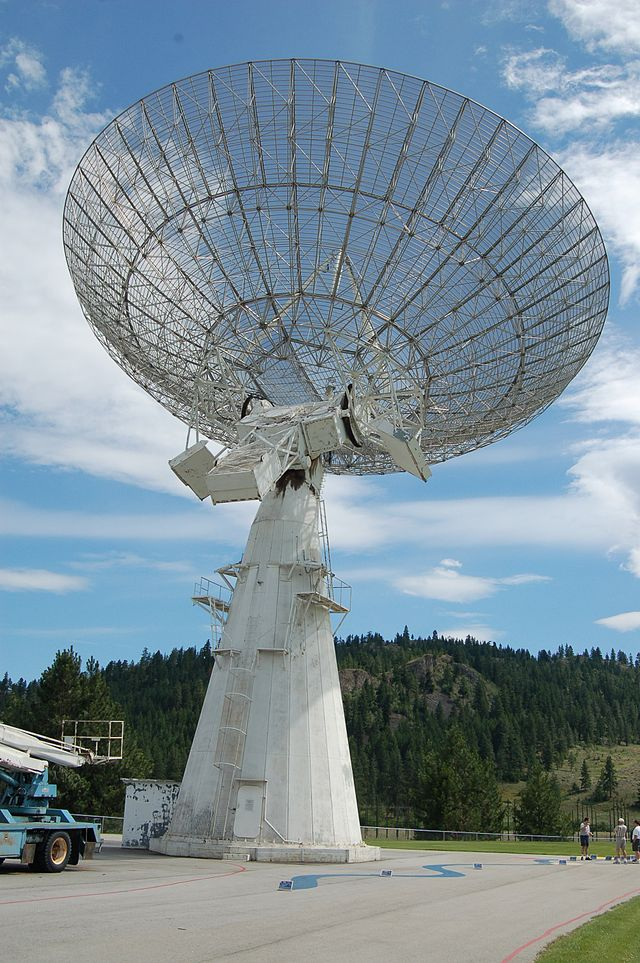
\includegraphics[width=1.2in]{Figures/DRAO_26m_dish.jpg}
\vspace{-0.5in}
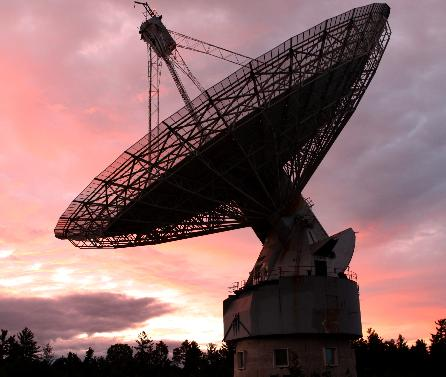
\includegraphics[width=1.9in]{Figures/IMG-7749-ARO-crop.JPG}
  }

  \frame{
\vspace{-0.5in}
    \frametitle{Canadian VLBI fringes!}
    \begin{itemize}
      \item work by Liam Connor, Robert Main
        \item crab giant pulse
        \item April 2016, ARO-DRAO
%          \vspace{-0.15in}
    \end{itemize}
\vspace{-0.1in}\hspace{.3in}
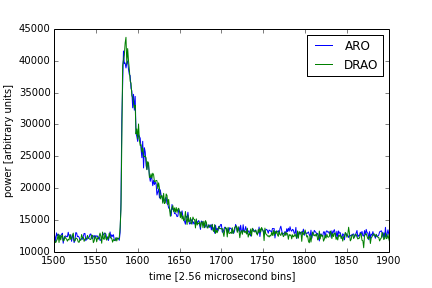
\includegraphics[width=1.9in]{Figures/ARO-DRAO-PulseComp.png}
\vspace{-0.5in}
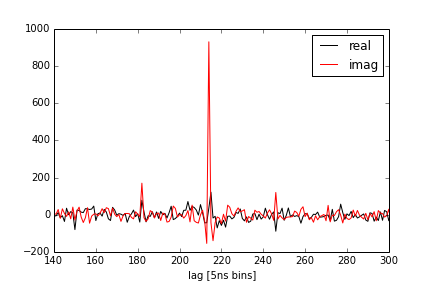
\includegraphics[width=1.9in]{Figures/ARO-DRAO-lf-zoom.png}
  }

  \frame{
    \frametitle{BGQ infrastructure}
    \begin{itemize}
        \item petabyte datasets software signal processing
        \item large linear algebra systems for phase retrieval solution
    \end{itemize}
}

  \frame{
    \frametitle{Partnership}
    \begin{itemize}
        \item grew from initial SOSCIP to CIFAR, OCE-CRD, CFI, ORF-RE, IDC
        \item partner institutes: Max Planck (Bonn), SJTU (Shanghai)
    \end{itemize}
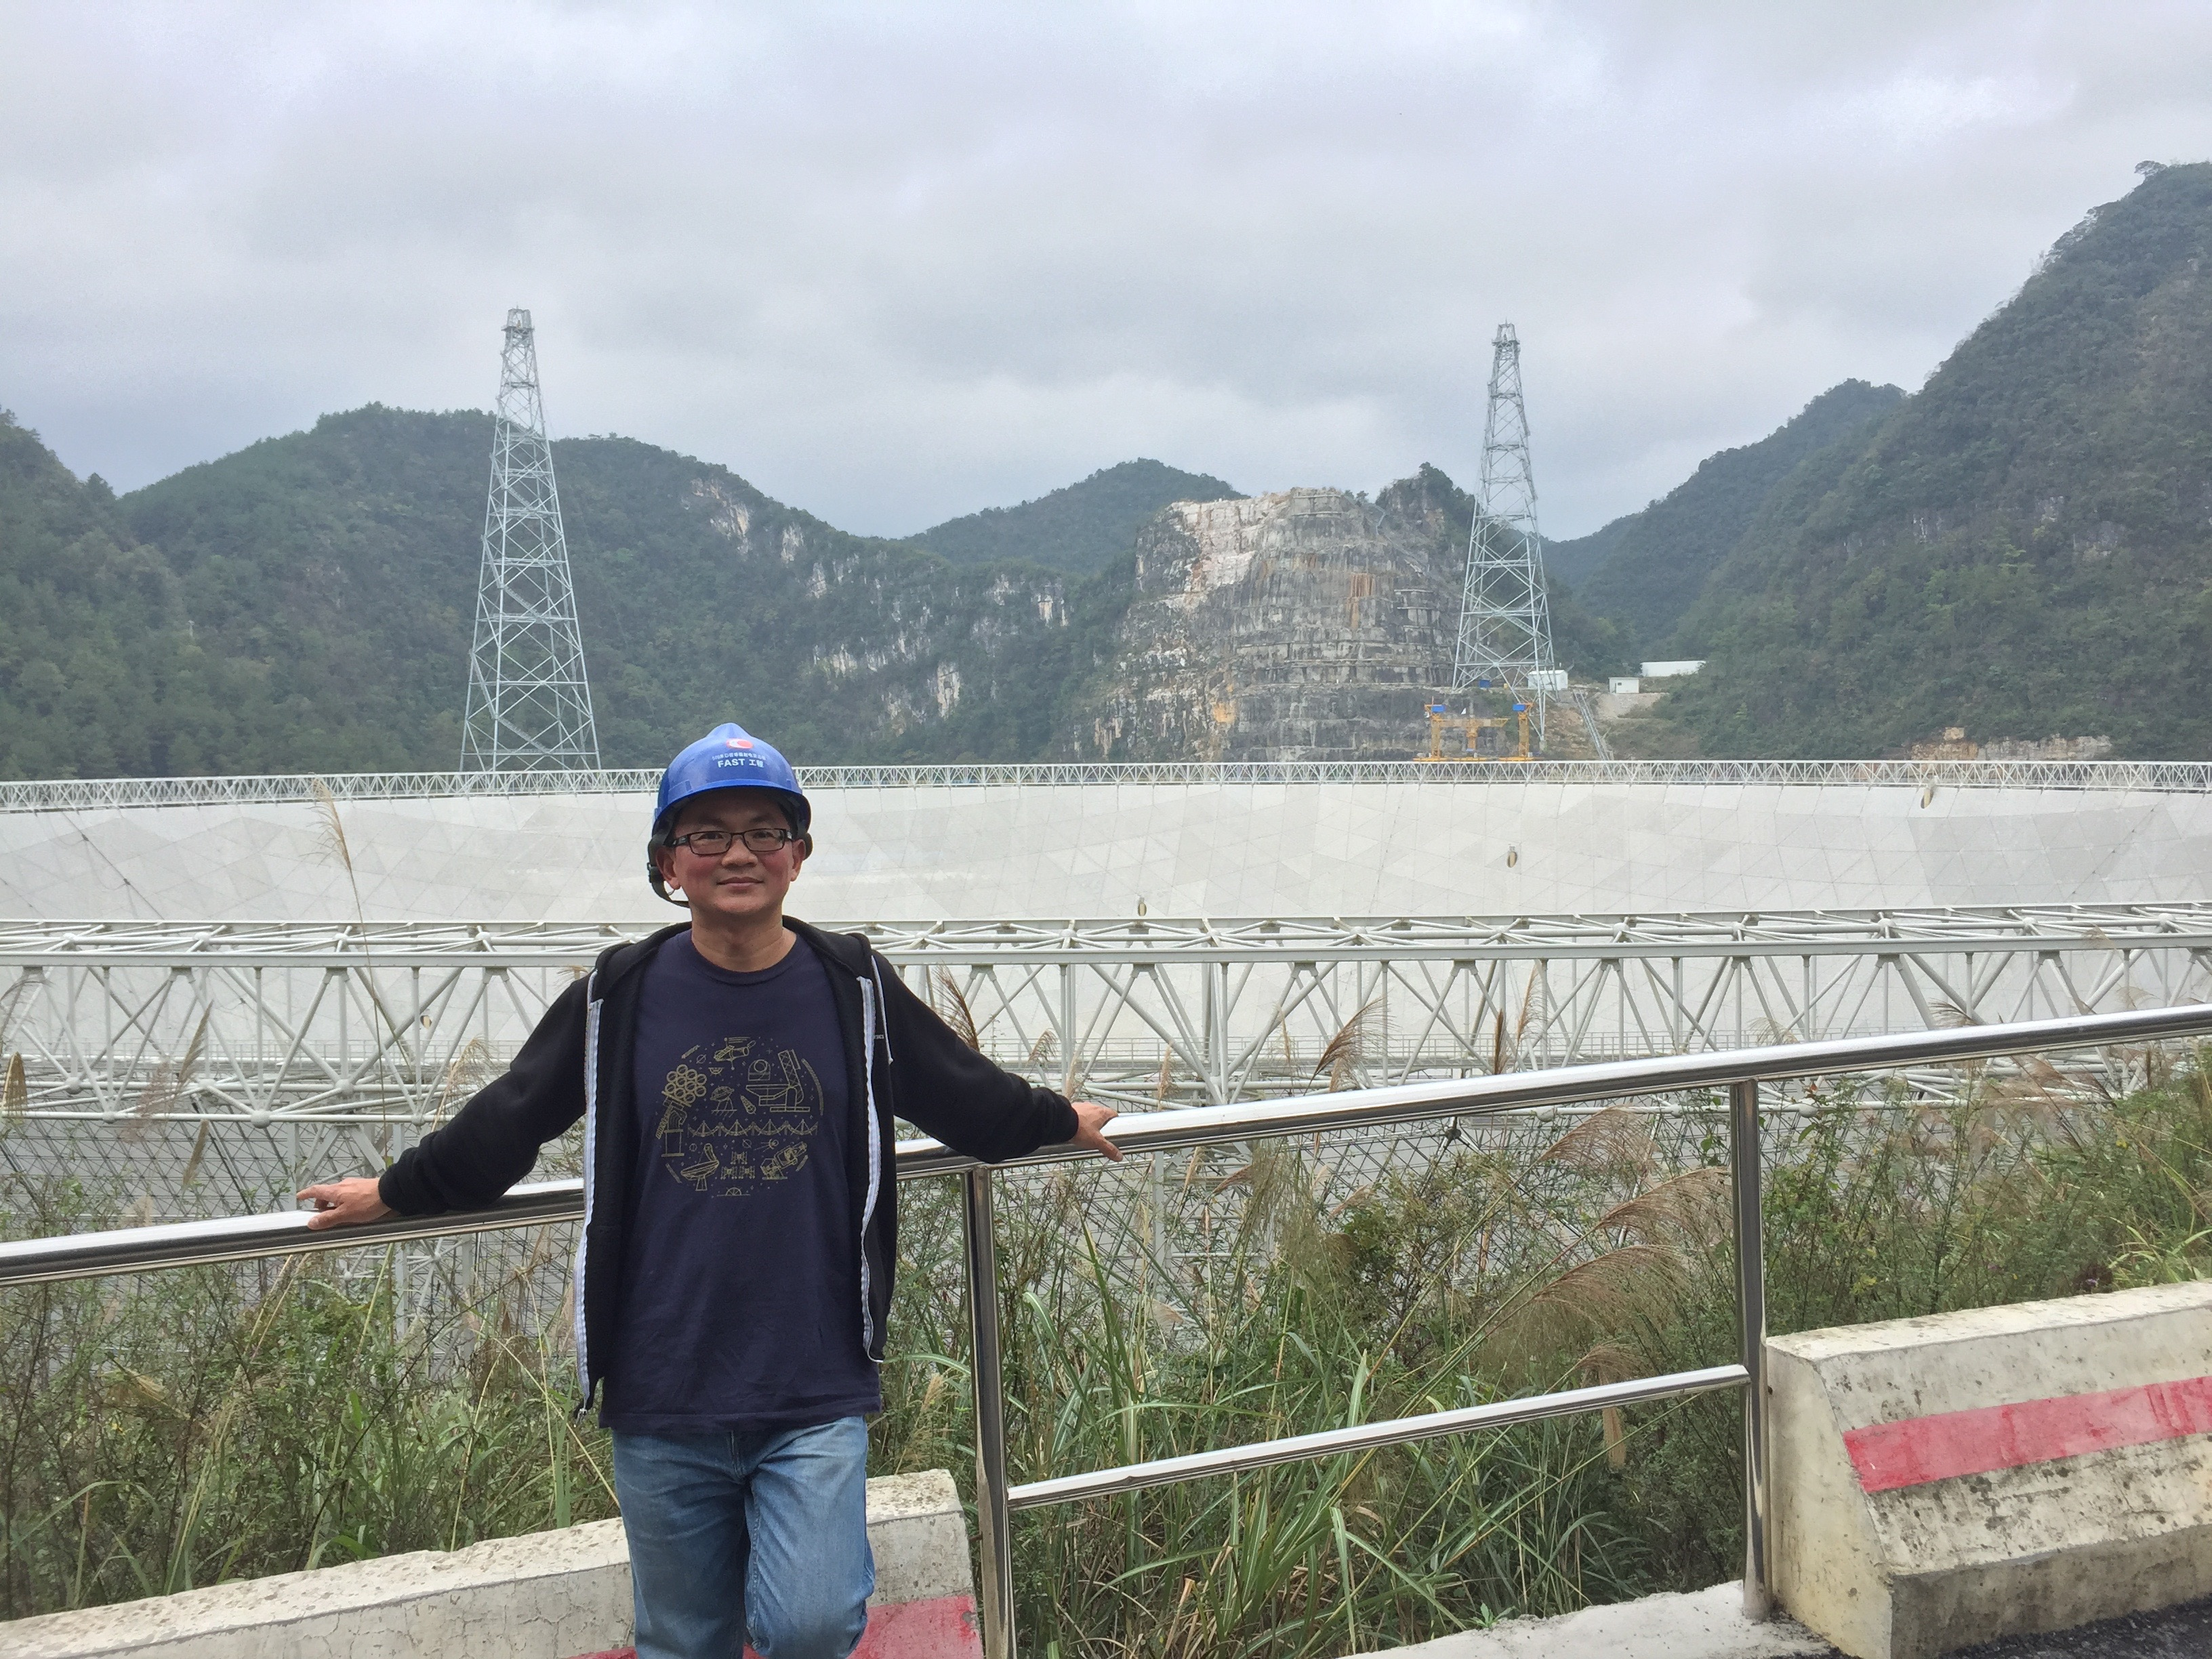
\includegraphics[width=1.9in]{Figures/fast_pen.jpg}
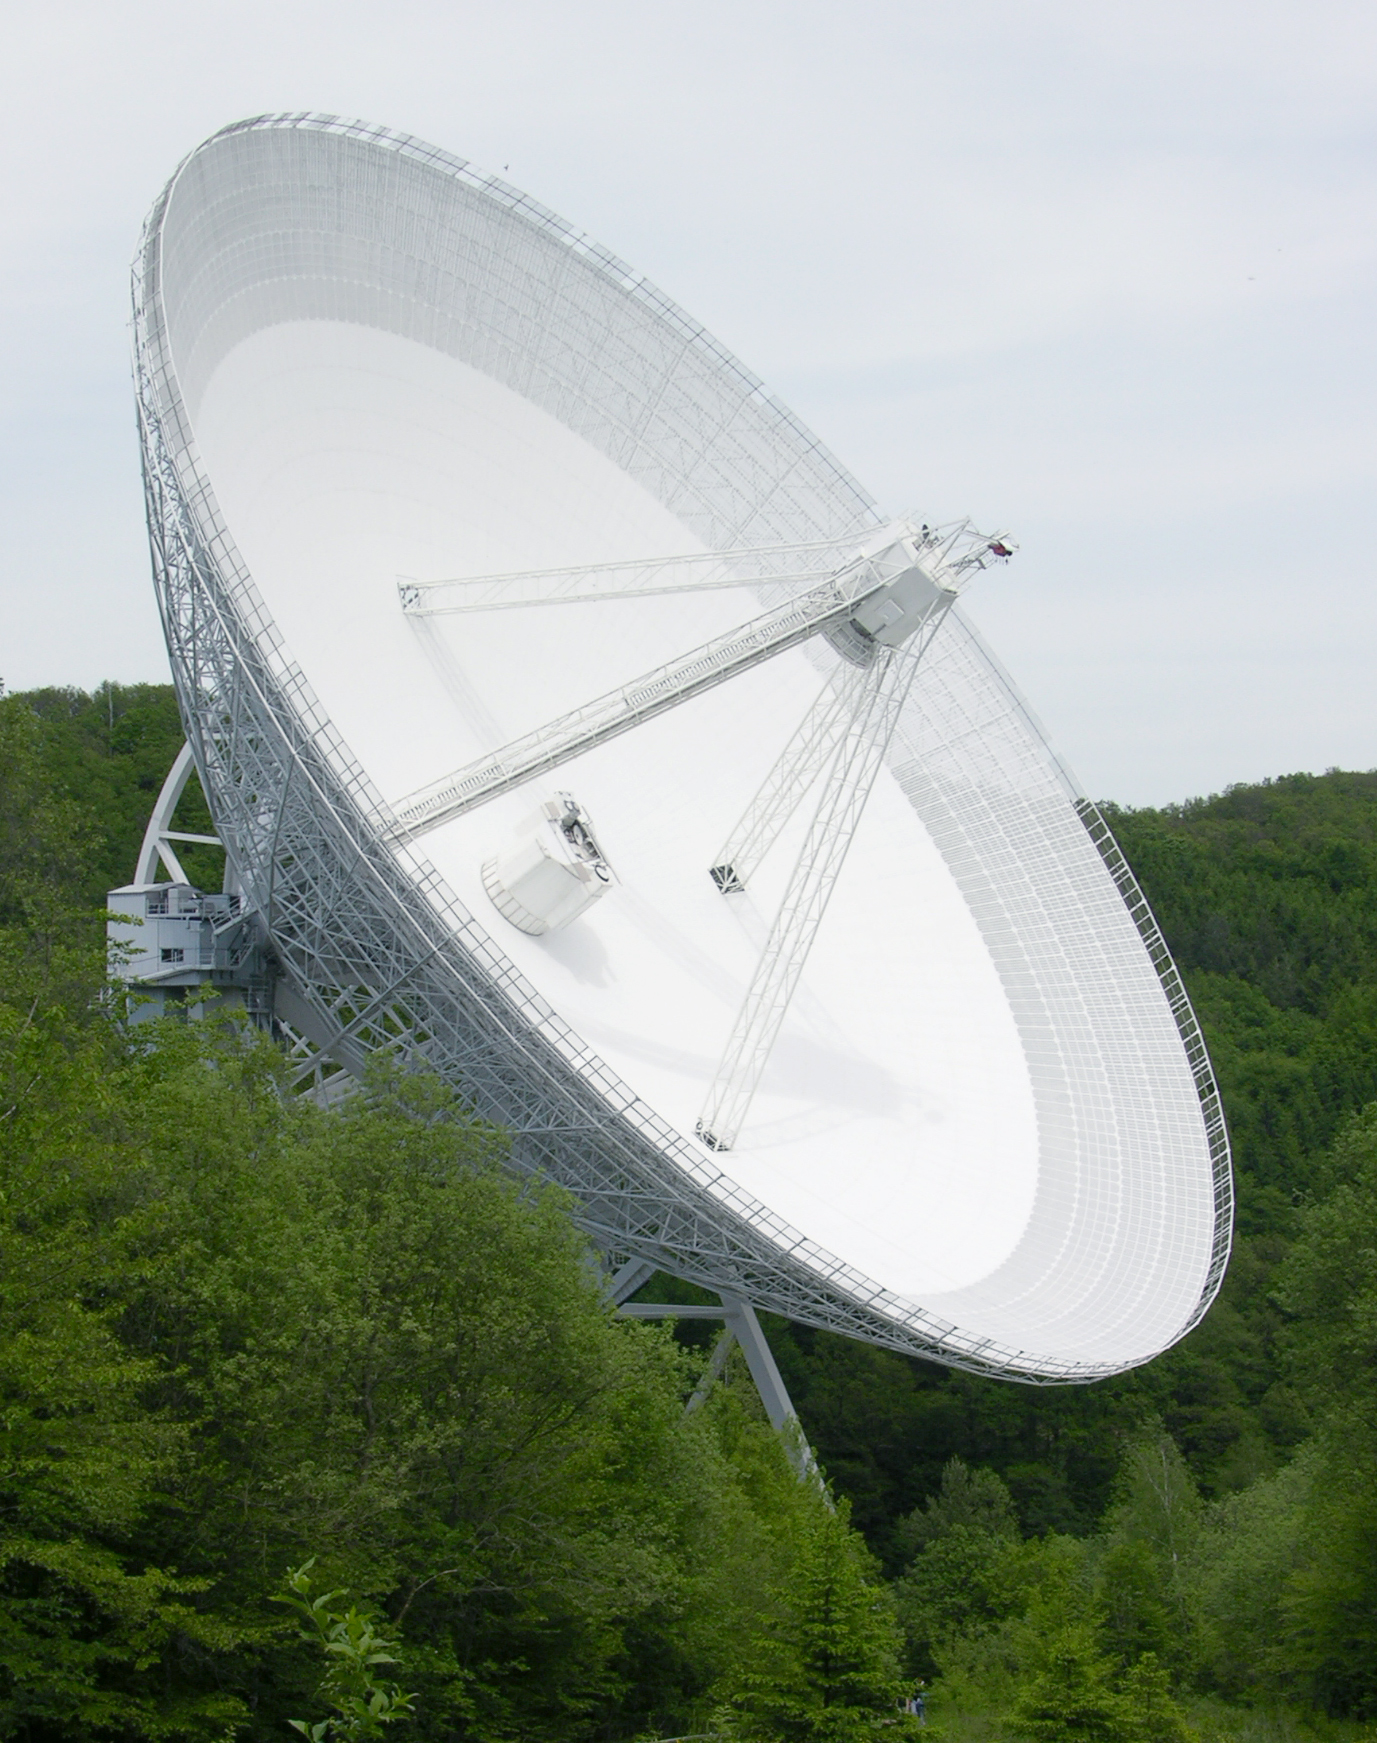
\includegraphics[width=1.5in]{Figures/DSCN6149_Effelsberg_totale.jpg}
}
\end{document}
